\section{Risikoabsch�tzung}
\begin{itemize}
\item Komplexit�t: Die Schnittstelle zu Lotus Notes kann schwierig zu realisieren sein.
\item Termin: Das Projekt wird nicht zum vereinbarten Termin abgeschlossen.
\item Qualit�t: Die vereinbarten Anforderungen werden nicht erf�llt.
\item Budget: Das Projekt wird teurer als geplant.
\end{itemize}

\subsection{Risiko - Eintrittswahrscheinlichkeit - Schadenpotenzial}

\begin{figure}
\begin{center}
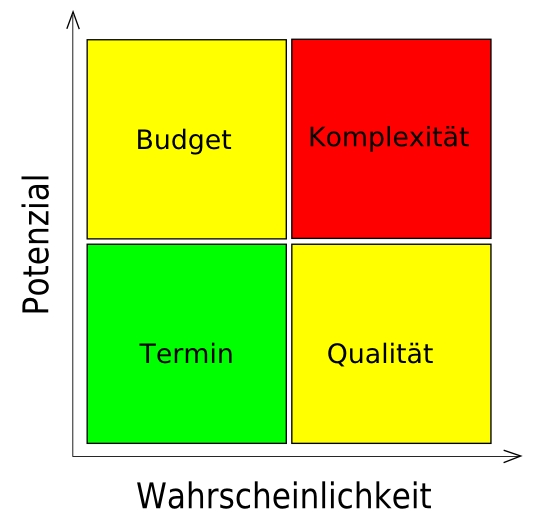
\includegraphics[width=0.8\textwidth]{abbildungen/Wahrscheinlichkeit-Potenzial.jpg}
\caption{Risiko - Eintrittswahrscheinlichkeit - Schadenpotenzial}
\end{center}
\end{figure}

\subsection{Risikomatrix}
\subsection{Vorbeugema�nahmen}
\subsection{Korrekturma�nahmen}